\chapter{Alternative Öffnungsmöglichkeiten}

\section{Sprachassistenten-Steuerung}
TODO

\section{Weboberfläche}
Da die Implementierung im Rahmen des Projekts jedoch auf einem Raspberry Pi stattfindet und Python bereits für viele Anwendungen innerhalb des Projekts verwendet wird, wird sich für das in Python geschriebene Webframework Flask entschieden. Dies hat den Vorteil, dass andere Komponenten, die bereits in Python geschrieben sind, direkt ohne Mehraufwand in die Weboberfläche integriert werden können.

Daher wird im Rahmen des Projekts für die Realisierung einer Weboberfläche eine einfache FlaskApp erstellt, die den üblichen Aufbau hat mit einer flaskapp.py, die die Weboberfläche steuert, und auf einzelne Templates, die wiederum in HTML geschrieben werden, zugreift. Hierbei wird in der flaskapp.py-Datei die Initialisierung der Weboberfläche sowie das Routing und dem Datentransfer zwischen den Seiten festgelegt sowie auch die Funktion, die die Garage öffnet. Als Templates die als Seite geladen werden, wird ein Template für die Startseite erstellt sowie ein Template für die Seite, auf der die Logs angezeigt werden sollen. Die Hauptseite, die bei Aufruf der Seite geladen wird, enthält einen Button, der mittels der in der flaskapp.py dafür festgelegten Funktion die SmartGarage öffnet und einen Eintrag in der Logs-Datei erstellt. Des Weiteren enthält diese Seite die Information ob in der Garage ein Fahrzeug steht, oder nicht. Dies geschieht über die Ultraschallmessung, wie bereits zuvor erläutert. Ebenfalls wird von dieser Seite aus auf die Logs-Seite verlinkt. Die Logs-Seite bezieht die Daten aus der Logs-Datei und gibt diese auf der Weboberfläche aus, wodurch der Besitzer der Garage die geloggten Öffnungen einsehen kann.

\section{RFID}
Die Implementierung eines RFID-Systems in der SmartGarage bietet eine weitere Möglichkeit die Garage zu öffnen. Für das Projekt wurde daher ein RFID-RC522 Modul an den Raspberry Pi angeschlossen, welches als Lesegerät Transponder auslesen kann. Angesteuert vom Raspberry Pi wird das Modul mittels der GPIO-Ports ähnlich wie beispielsweise bereits dem Ultraschallsensors. Das Auslesen wird dann mit Hilfe eines Python-Skripts gesteuert und mit einer Whitelist abgeglichen.

Als Transponder kann im Projekt jede beschreibbare RFID-Karte oder RFID-Chipkarte verwendet werden, solange diese die vorausgesetzte Frequenz von 13,56MHz unterstützt. Im Projekt wird hierfür eine RFID-Karte, die nicht mit dem richtigen Code beschriftet ist, als Beispiel für eine fehlerhafte Identifikation verwendet. 

\section{Ultraschallsensor}
TODO voherigen Teil aufsplitten, Quelle

\section{Piezo-Lautsprecher}
Bei der Umsetzung des Akustischen Signal Tons der Anlage wurde provisorisch auf einen sogenannten aktiven Summer zurückgegriffen. Dieser erklingt zum Beispiel, wenn der Richtige RFID Chip an das Lesegerät gehalten wird und somit die Garage geöffnet oder geschlossen wird. Dabei handelt es sich um ein Oszillator der, wird er einer gewissen Spannung untersetzt, anfängt zu Vibrieren und damit ein Ton erzeugt. Ausgeführt und koordiniert wird der Buzzer über ein Simples Python Skript das mittels der Bibliothek GPIO (General-Purpose Input/Output) in der Lage ist den Buzzer an oder auszuschalten. Dabei wird durch einen definierten Port, in diesem Fall „Port 4“, mittels einer $for$ Schleife die Spannung je nach $positivem$ oder $negativem$ Signal Ton koordiniert und eine andere Tonsequenz abgespielt. 


\section{Steckplan}

Auf Abbildung \ref{Steckplansm} ist die schlussendlich verwendete Steckung abgebildet. Hierbei war zu beachten, dass die im Internet verfügbaren Anleitungen und Tutorials nicht unbedingt miteinander kompatibel sind und einige \ac{GPIO}-Pins von mehreren Vorlagen verwendet werden. Hier muss demetsprechend ein anderer freier Pin mit gleicher I/O-Funktion gefunden werden und der Code angepasst werden. Außerdem ist die Spannung zwingend zu beachten. Manche Module, wie der Ultraschallsensor, benötigen eine Spannung von 5V, andere nur 3.3V. Ein versehentliches Verbinden der beiden Spannungsnetze kann zu irreperablen Hardwareschäden führen. 
Der dazugehörge elektrische Schaltplan findet sich in Anhang \ref{Schaltplan}
\begin{figure}[H]
	\centering 
	\label{Steckplansm}
	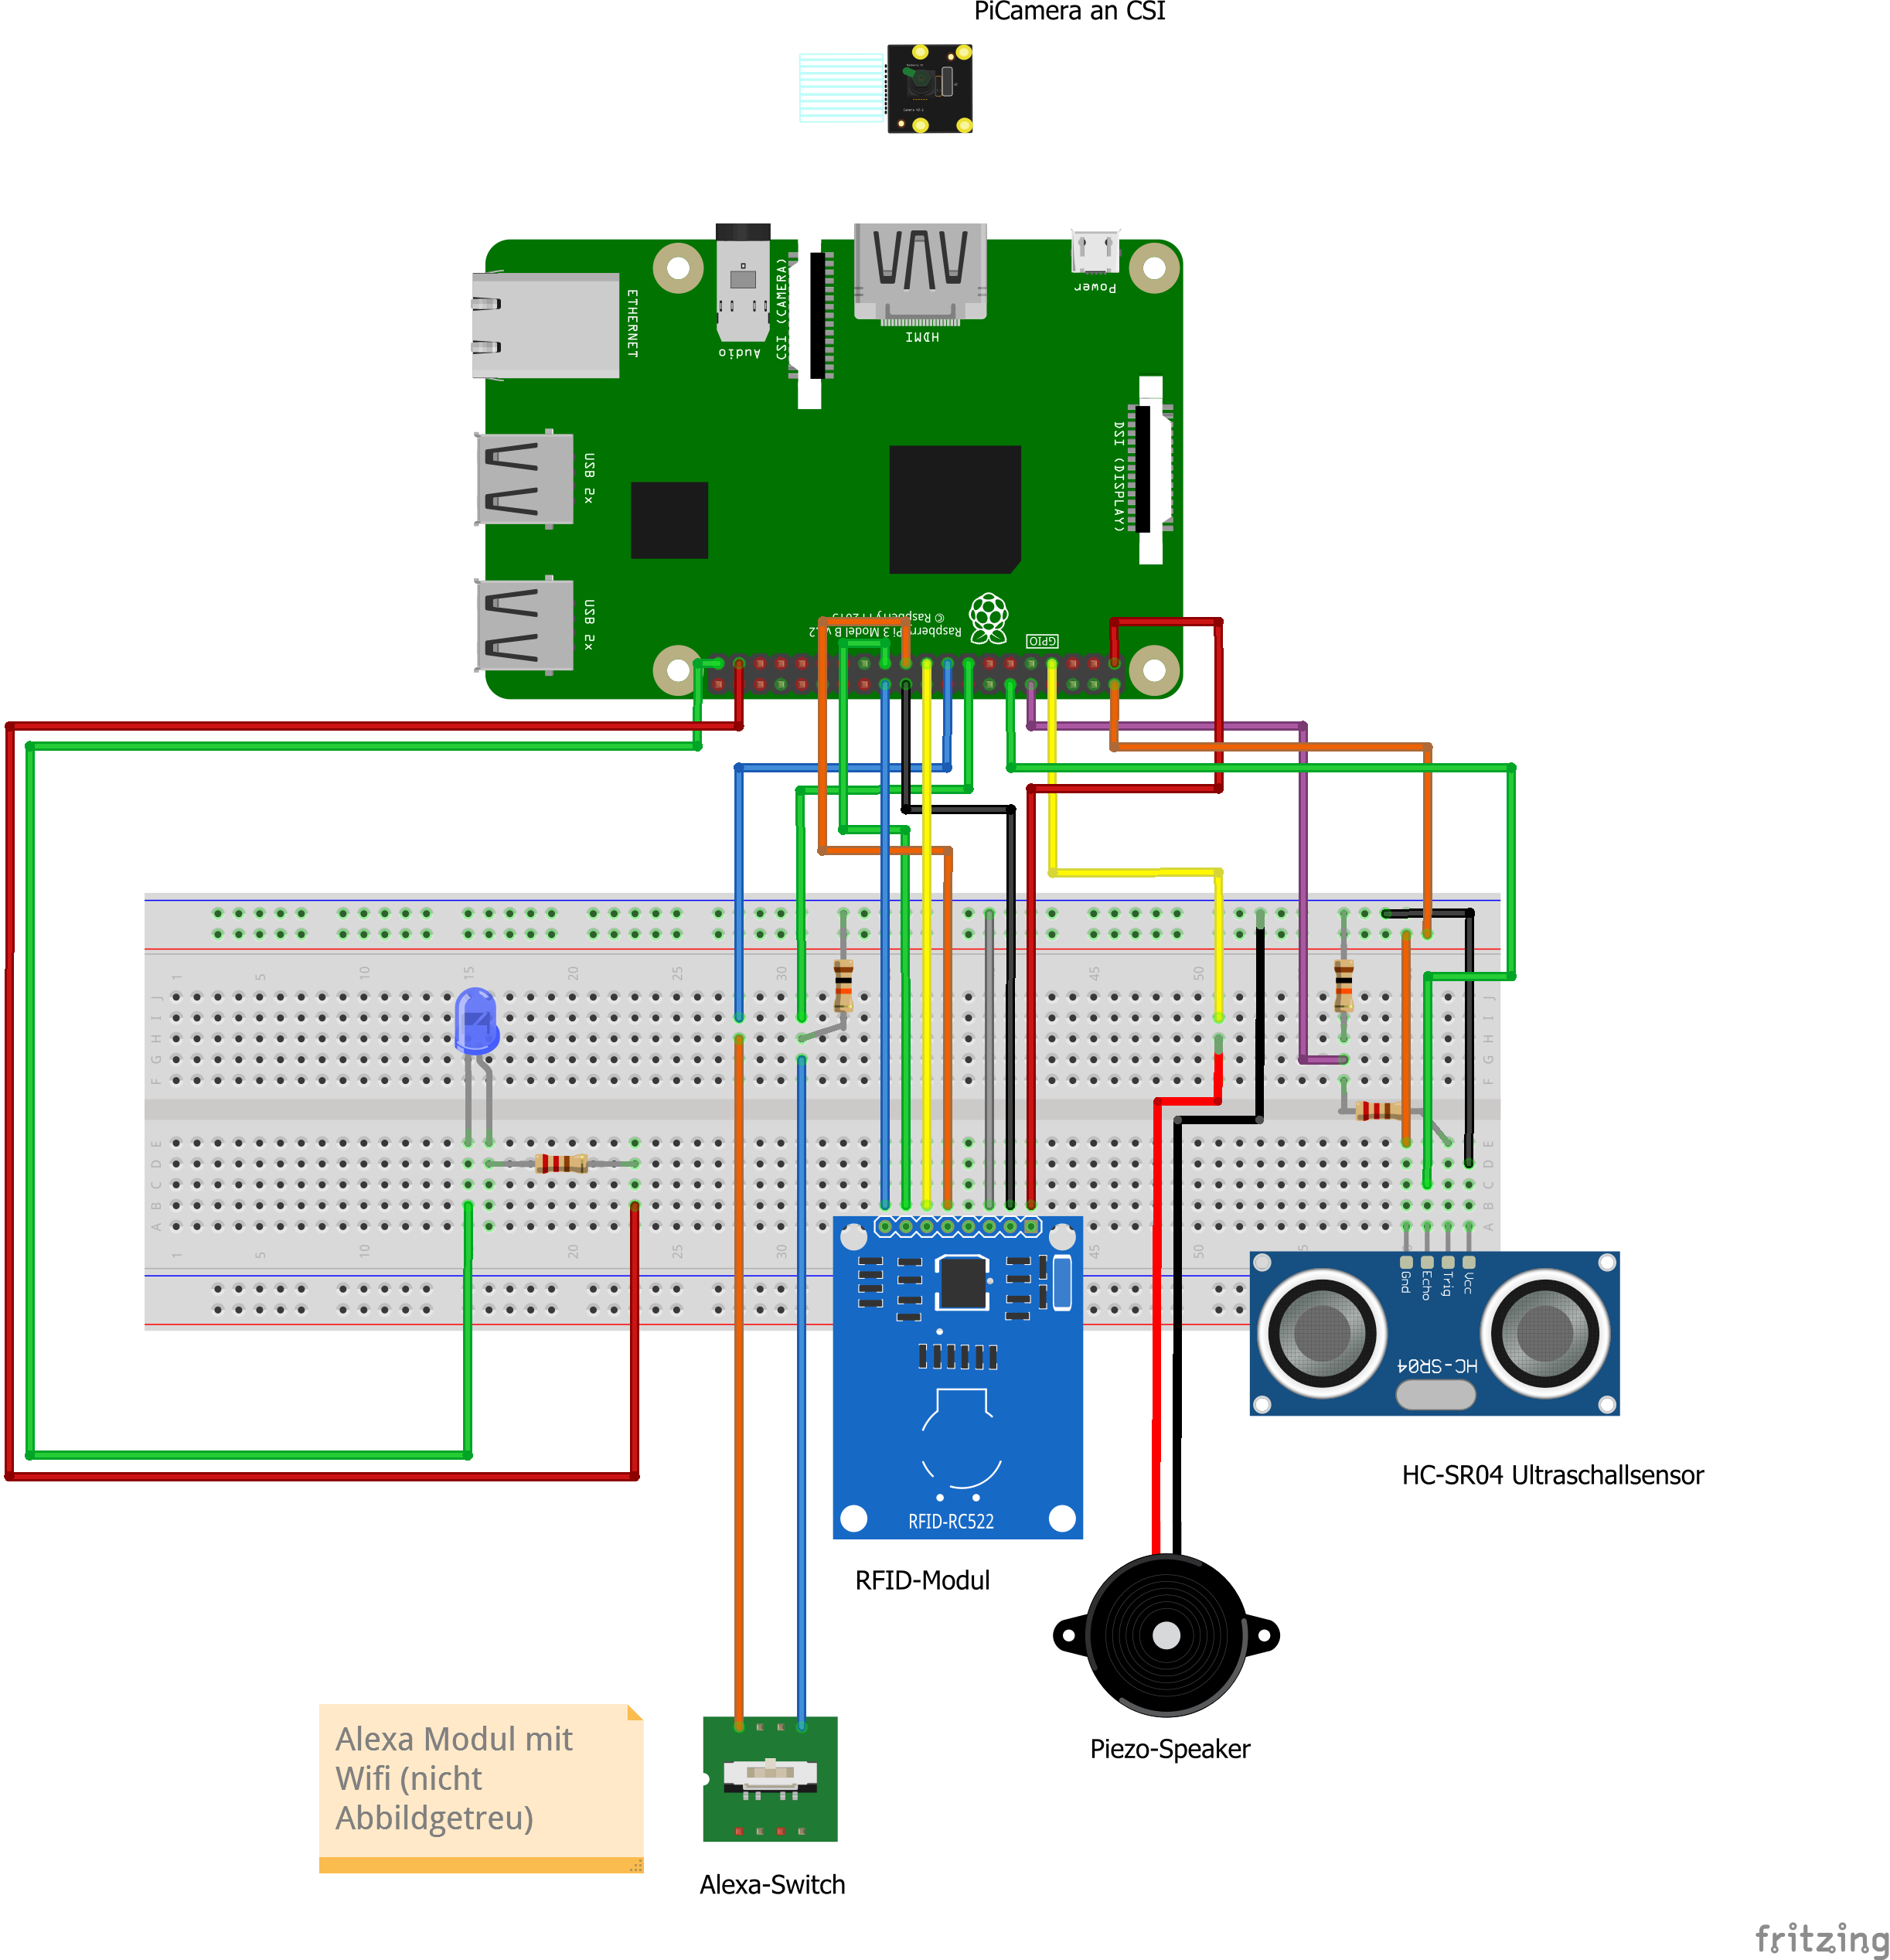
\includegraphics[scale=0.75]{\imagedir/SmartGarage.png}
	\captionsetup{format=hang}
	\caption[Steckplan]{\label{Steckplansm}Steckplan der gesamten Hardware \\Quelle: Eigene Darstellung}
\end{figure}\section{Schaltlogik}
Hier nochmal erklären oder selbsterklärendes Bild einfach in den Anhang
\begin{figure}[H]
	\centering 
	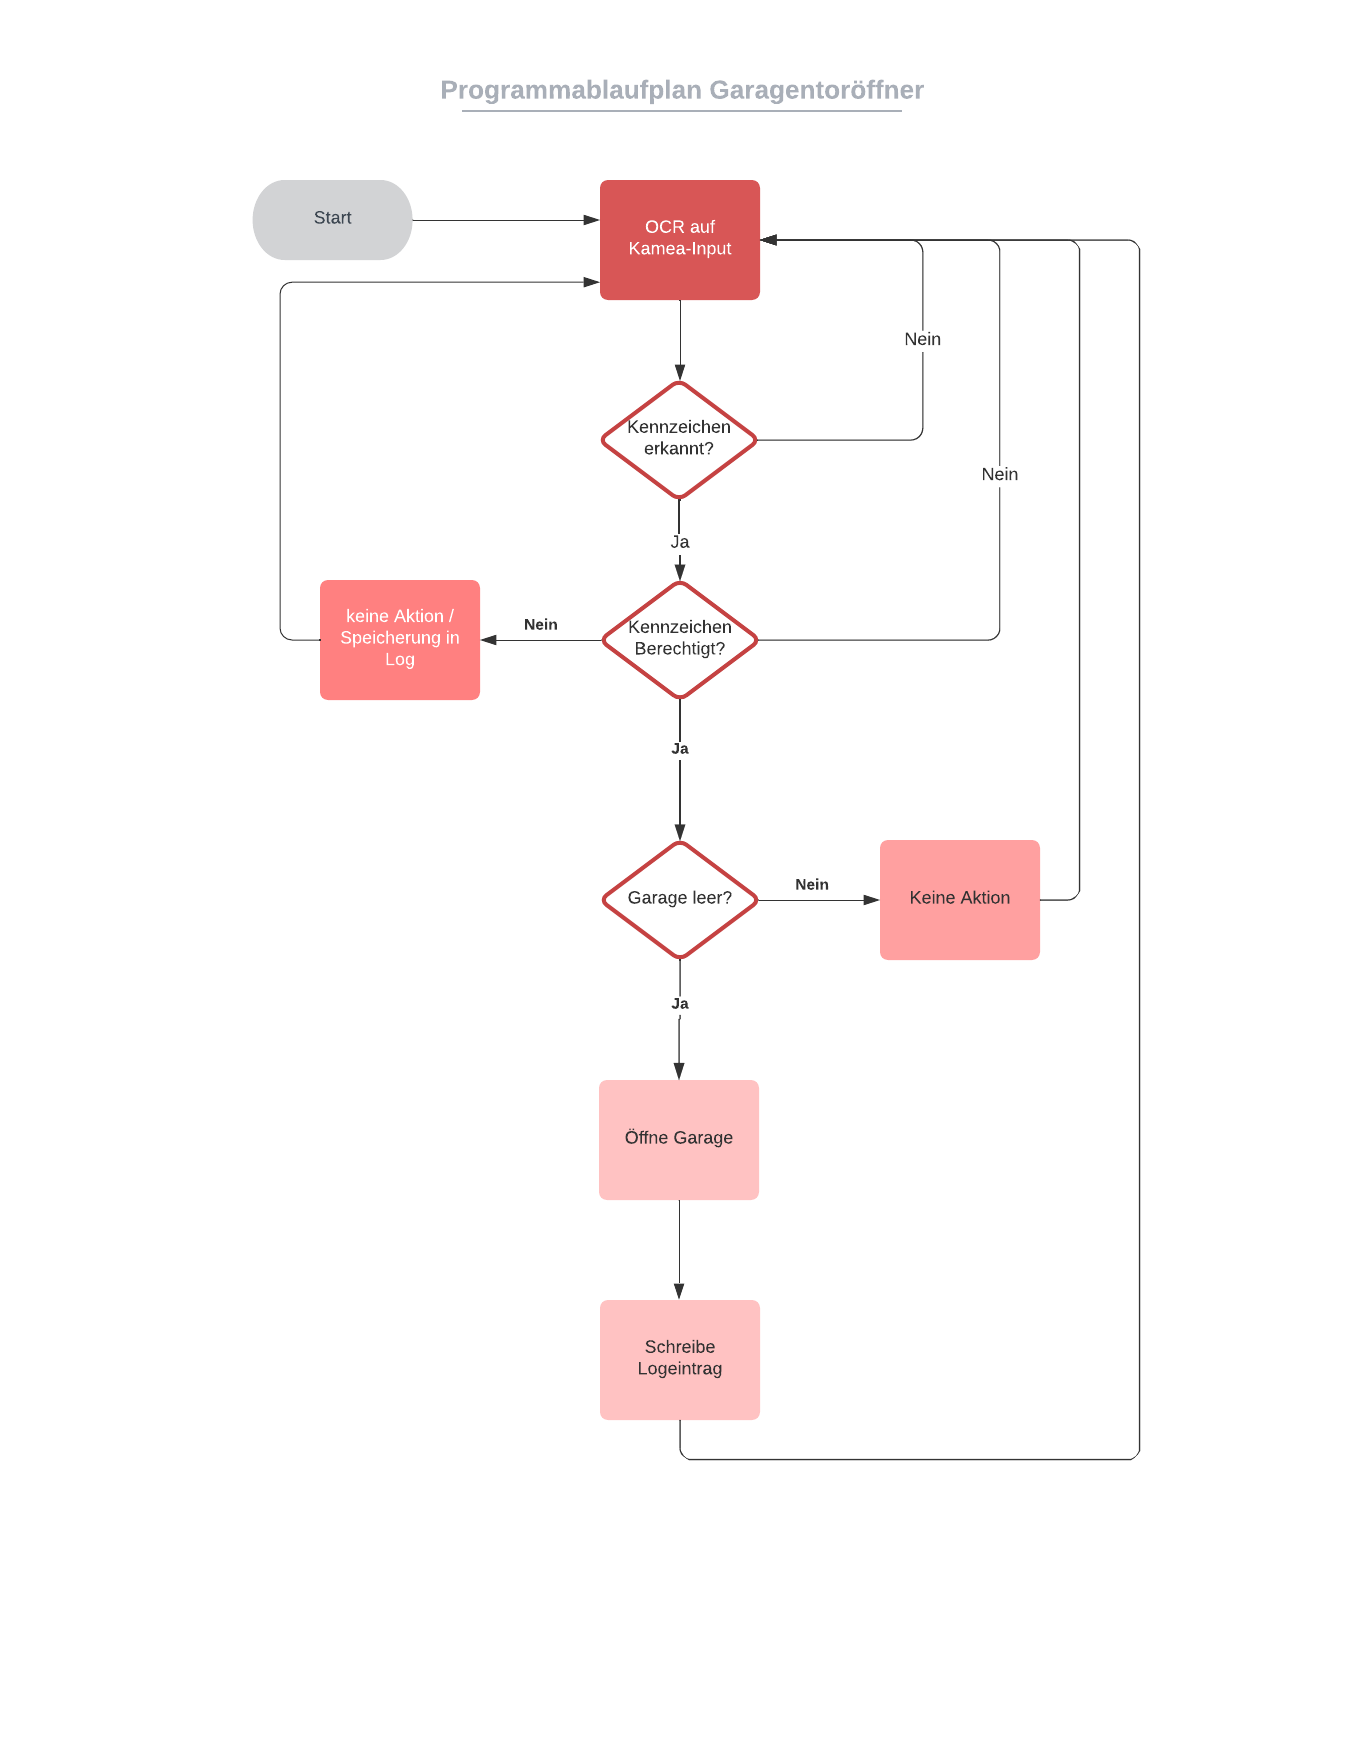
\includegraphics[scale=0.75]{\imagedir/Programmablaufplan.png}
	\captionsetup{format=hang}
	\caption[Programmablauf]{\label{fig:test}Ablauf der Kennzeichenerkennungs-Schleife \\Quelle: Eigene Darstellung}
\end{figure}
\chapter{Risiken und Limitierungen}

Mehrere problematische Punkte konnten innerhalb der relativ kurzen Projektlaufzeit noch nicht ausreichend adressiert werden. 

Zum einen hat die verwendete Software noch Schwierigkeiten mit Störungen durch Fahrzeug- und Kennzeichenhalterbeschriftungen und deutsche Umlaute, die in manchen Kennzeichen vorhanden sind, können noch nicht erkannt werden. Dies war auf den erfassten Testdaten in Mannheim/Heidelberg nicht nicht problematisch, wird es aber für andere Regionen sein.
Zum anderen ergeben sich natürlich durch die optische Erkennung etliche Probleme bei erschwerten Sichtverhältnissen wie Schnee, Regen, Dunkelheit oder schlicht verschmutzten Kennzeichen. 

Ein weiterer bedeutender Punkt ist die mangelnde Sicherheit des Systems. Da die Öffnung des Garagentors nur durch das Kennzeichen geschieht, ist das Missbrauchs-Bzw. Einbruchspotenzial groß.

\chapter{Wirtschaftliche Aspekte}
Auch wenn die technische Konzeption und Umsetzung im Mittelpunkt dieser Arbeit stehen, soll aufgrund der Ausrichtung des Studiengangs hier kurz auf einige betriebswirtschaftliche Aspekte des Projekts eingegangen werden.\subparagraph*{Entwicklungskosten}
   \newline
Pro Teammitglied

\begin{tabular}[h]{lcr}
2x Projektkonzeption/Kick-Off online 2 Stunden \\
3x Workshops a 12 Stunden\\
1x Workshop a 8 Stunden\\
1x Praxistest 4 Stunden\\
1x Abschluss-Workshop a 24 Stunden \\
8 Stunden Ausarbeitung Projektbericht / Dokumentation\\
\end{tabular} \newline

Bei einem angenommenen Stundenlohn von 15€, der für Werkstudenten mit vergleichbaren Kenntnissen angemessen ist, ergibt sich bei 336 Mannstunden geschätzte kalkulatorische Entwicklungskosten von 5040€
\subparagraph*{Materialkosten} in Euro, inkl. Versand  \newline  %\footnote{Alle Preise in €, inkl. Versand}

\begin{tabular}[h]{lcr}
Raspberry Pi 3	&   39,95 \autocite{Pi3b} \newline \\
RFID-Modul RC552 &		5,00\autocite{RFID} \newline\\
Ultraschallmodul	&  8,94\autocite{SR04} \newline \\
Amazon Alexa Wifi Modul & 13,99\autocite{eWe}	\\
OAK-D Kamera & 185,51 \\
\textbf{Summe}			&	\textbf{253,39}
\end{tabular} \newline


Die geschätzte Installationszeit pro Einheit für Verkabelung des Kameramoduls und des RasPi, Befestigung des RFID-Sensors, Ausrichtung der Kamera und Tests beträgt für einen geübten Elektriker ca. 4 Stunden.
Bei einem angenommenen Kosten von 60€/Stunde wären dies 240€ (ohne Anfahrt). Der Verkaufspreis inklusive Installation müsste also mindestens bei knapp 500€ liegen, um einen Deckungskostenbeitrag zu erzielen und die Entwicklungskosten von 5040€ zu decken.




